\documentclass[fr]{../../../../../../eplexam}
\usepackage{../../../../../../eplchem}
\usepackage{../../../../../../eplunits}

\hypertitle{Chimie et chimie physique}{3}{FSAB}{1302}{2013}{Août}{All}
{Martin Braquet}
{Hervé Jeanmart, Christian Bailly et Francis Delannay}

\section{Cycle}

Une habitation est chauffée grâce à une pompe à chaleur fonctionnant selon un cycle de Carnot parcouru dans le sens récepteur. Le système qui parcourt le cycle est fermé et contient de l’air (gaz parfait). La température extérieure est de 4$^\circ$C. Dans ces conditions, la puissance
thermique nécessaire pour maintenir la température de l’habitation à 19$^\circ$C est de 10kW.

\begin{enumerate}

\item Sachant que la fréquence à laquelle le cycle est parcouru par le système fermé est de 25 Hz, complétez le tableau suivant

\[
      \begin{tabular}{|c|cccc|}
        \hline
        & $p[\si{\bar}]$ & V[$m^3$] & $T[\si{\kelvin}]$ & $S-S_1[J/K]$\\
        \hline
        1$^*$ & 1 & &  & \\
        \hline
        2 &  &  &  & \\
        \hline
        3 & 2 &  &  & \\
        \hline
        4 &  &  &  & \\
        \hline
      \end{tabular}
\]
\textit{*Le point 1 correspond à l’état du système où la pression est minimale.}

\item Quelle est la puissance mécanique nécessaire pour alimenter la machine ?

\item Dessinez les diagrammes (p,V) et (T,S) du cycle.

\end{enumerate}

\begin{solution}

\begin{enumerate}

\item 
Les transformations d'un cycle de Carnot récepteur (inversé) sont:
\begin{itemize}
    \item 1 $\to$ 2: compression adiabatique
    \item 2 $\to$ 3: compression isotherme
    \item 3 $\to$ 4: détente adiabatique
    \item 4 $\to$ 1: détente isotherme
\end{itemize}

On rappelle aussi que:
$$ c_p=\frac{7}{2}R \qquad c_v=\frac{5}{2}R \qquad \gamma=1,4$$
La température extérieure correspond aux états 1 et 4 puisqu'elle s'élève lors de la compression adiabatique.

On détermine les pressions par
$$\bigg(\frac{p_2}{p_1}\bigg)=\bigg(\frac{T_2}{T_1}\bigg)^{\frac{\gamma}{\gamma-1}}$$
$$p_2= 1\bigg(\frac{292}{277}\bigg)^{\frac{\gamma}{\gamma-1}}=1,2027\:[bar]$$
$$p_4= 2\bigg(\frac{277}{292}\bigg)^{\frac{\gamma}{\gamma-1}}=1,6629\:[bar]$$
On a donc ce tableau-ci:

\[
      \begin{tabular}{|c|cccc|}
        \hline
        & $p[\si{\bar}]$ & V[$m^3$] & $T[\si{\kelvin}]$ & $S-S_1[J/K]$\\
        \hline
        1$^*$ & 1 &  & 277 & \\
        \hline
        2 & 1,2027 &  & 292 & \\
        \hline
        3 & 2 &  & 292 & \\
        \hline
        4 & 1,6629 &  & 277 & \\
        \hline
      \end{tabular}
\]

La chaleur dégagée à la source chaude au cours d'un cycle vaut
$$Q_{HOT}=-\frac{P_{therm}}{f}=\frac{-10000}{25}=-400\:J.$$

En considérant la compression isotherme de ce cycle:
$$-400=Q_{2-3}=-W_{2-3}
=nRT_2\ln\frac{V_3}{V_2}
=nRT_2\ln\frac{p_2}{p_3}$$
puisque $V_3/V_2=(p_2/p_3)$ pour une transformation isotherme.
$$\Rightarrow n=\frac{-400}{8,3145*292\ln\frac{1,2027}{2}}=0,3239\:mol$$
On en déduit les volumes:
$$V_i=\frac{nRT_i}{p_i}$$
$$\Rightarrow V_1=0,007461 \:[m^3]$$
$$V_2= 0,00654 \:[m^3]$$
$$V_3=0,003933  \:[m^3]$$
$$V_4=0,004487  \:[m^3]$$

Les variations d'entropie sont données par:
$$S_2-S_1=0$$
$$S_3-S_2=\int_2^3\frac{\delta Q}{T}=\frac{Q_{2-3}}{T_2}=\frac{400}{292}=-1,37 \:[J/K]$$
$$S_4-S_3=0$$
$$S_1-S_4=nR\ln\frac{V_1}{V_4}=1,37 \:[J/K]$$

Le tableau final est donné ci-dessous.

\[
      \begin{tabular}{|c|cccc|}
        \hline
        & $p[\si{\bar}]$ & V[$m^3$] & $T[\si{\kelvin}]$ & $S-S_1[J/K]$\\
        \hline
        1$^*$ & 1 & 0,007461 & 277 & 0\\
        \hline
        2 & 1,2027 & 0,00654 & 292 & 0\\
        \hline
        3 & 2 & 0,003933 & 292 & -1,37\\
        \hline
        4 & 1,6629 & 0,004487 & 277 & -1,37\\
        \hline
      \end{tabular}
\]

\item La puissance mécanique nécessaire pour alimenter la machine correspond à 
$$P_{\mbox{méca}}=fW_{tot}=f|Q_{tot}|=f\Delta T \Delta S=25*15*1,37=514\:W$$

\item 

	\begin{solfig}{C}{Diagrammes (p,V) et (T,S)}
    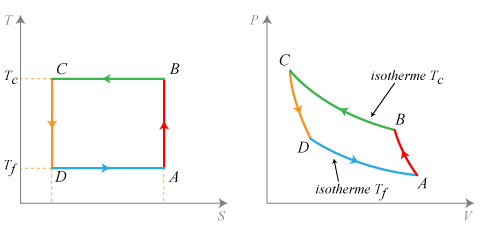
\includegraphics[scale=0.9]{Carnot.png}
	\end{solfig}

\end{enumerate}

\end{solution}

\end{document}
